\documentclass{article}\usepackage[]{graphicx}\usepackage[]{color}
%% maxwidth is the original width if it is less than linewidth
%% otherwise use linewidth (to make sure the graphics do not exceed the margin)
\makeatletter
\def\maxwidth{ %
  \ifdim\Gin@nat@width>\linewidth
    \linewidth
  \else
    \Gin@nat@width
  \fi
}
\makeatother

\definecolor{fgcolor}{rgb}{0.345, 0.345, 0.345}
\newcommand{\hlnum}[1]{\textcolor[rgb]{0.686,0.059,0.569}{#1}}%
\newcommand{\hlstr}[1]{\textcolor[rgb]{0.192,0.494,0.8}{#1}}%
\newcommand{\hlcom}[1]{\textcolor[rgb]{0.678,0.584,0.686}{\textit{#1}}}%
\newcommand{\hlopt}[1]{\textcolor[rgb]{0,0,0}{#1}}%
\newcommand{\hlstd}[1]{\textcolor[rgb]{0.345,0.345,0.345}{#1}}%
\newcommand{\hlkwa}[1]{\textcolor[rgb]{0.161,0.373,0.58}{\textbf{#1}}}%
\newcommand{\hlkwb}[1]{\textcolor[rgb]{0.69,0.353,0.396}{#1}}%
\newcommand{\hlkwc}[1]{\textcolor[rgb]{0.333,0.667,0.333}{#1}}%
\newcommand{\hlkwd}[1]{\textcolor[rgb]{0.737,0.353,0.396}{\textbf{#1}}}%

\usepackage{framed}
\makeatletter
\newenvironment{kframe}{%
 \def\at@end@of@kframe{}%
 \ifinner\ifhmode%
  \def\at@end@of@kframe{\end{minipage}}%
  \begin{minipage}{\columnwidth}%
 \fi\fi%
 \def\FrameCommand##1{\hskip\@totalleftmargin \hskip-\fboxsep
 \colorbox{shadecolor}{##1}\hskip-\fboxsep
     % There is no \\@totalrightmargin, so:
     \hskip-\linewidth \hskip-\@totalleftmargin \hskip\columnwidth}%
 \MakeFramed {\advance\hsize-\width
   \@totalleftmargin\z@ \linewidth\hsize
   \@setminipage}}%
 {\par\unskip\endMakeFramed%
 \at@end@of@kframe}
\makeatother

\definecolor{shadecolor}{rgb}{.97, .97, .97}
\definecolor{messagecolor}{rgb}{0, 0, 0}
\definecolor{warningcolor}{rgb}{1, 0, 1}
\definecolor{errorcolor}{rgb}{1, 0, 0}
\newenvironment{knitrout}{}{} % an empty environment to be redefined in TeX

\usepackage{alltt}
\usepackage{graphicx, hyperref}
\usepackage[backend=bibtex, natbib=true]{biblatex}
\addbibresource{references/refs.bib}

\usepackage{color}
\newcommand{\hh}[1]{{\color{magenta} #1}}
\IfFileExists{upquote.sty}{\usepackage{upquote}}{}




\begin{document}

\section{Background}
\subsection{Networks}
\subsection{Visualization}
\subsection{Layout Algorithms}

\section{User Interface}
\subsection{Design and Functionality}

\subsection{Technical Aspects}
\subsubsection{Software}

gravicom utilizes three main pieces of software to establish interactive user control of a random graph as sketched out in figure~\ref{fig:clientserver}. The three pieces used are Shiny, D3, and igraph. They are used to manage server/client interaction, user interface and graph layout, and data formatting, respectively.

\begin{figure}[hbtp]
\centering
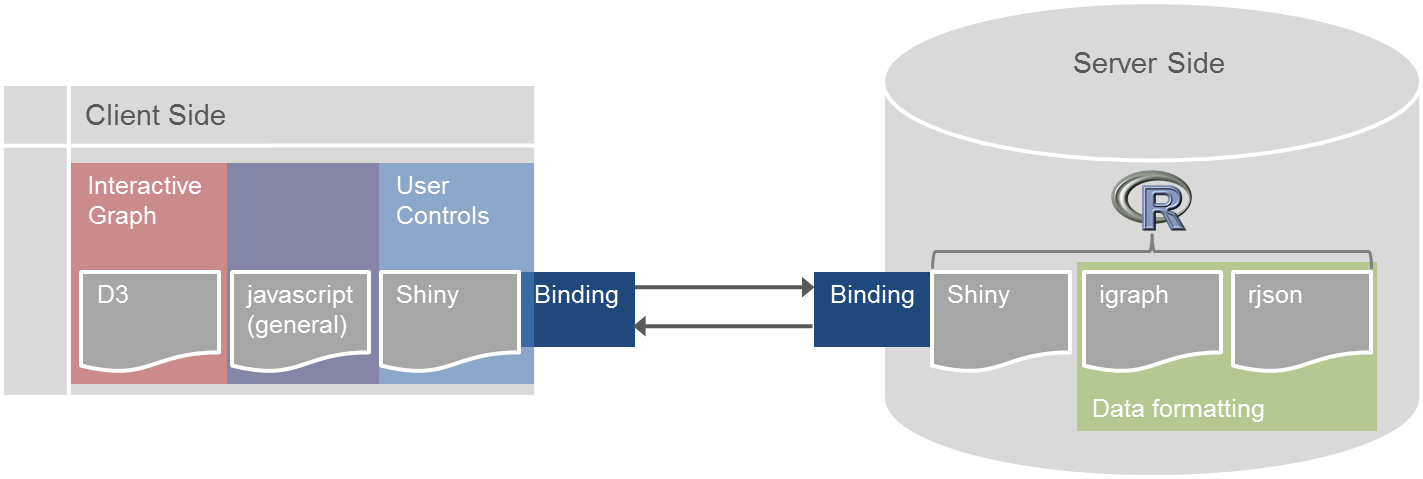
\includegraphics[width=\textwidth]{images/clientserverflow.png}
\caption{\label{fig:clientserver} Relationship between client and server, specifically focusing on how data travels between the two.}
\end{figure}

There are very minimal software requirements for a user of gravicom. The client simply needs to have a \hh{Javascrip enabled internet} browser, \hh{something} which \hh{almost any modern browser fulfills} (\hh{an exception is} IE8 and below). 

The server side requirements are more extensive, but this does not affect the user of gravicom, only those wanting to host their own instance of the application. To host gravicom, a Linux server is required, with the following installed:

\begin{itemize}
\item Node.js (0.8.16 or later)
\item {\tt R} (2.15 or later)
\item Shiny {\tt R} package, installed into the machine-wide site library. 
\item Shiny Server
\end{itemize}


\paragraph{Shiny}

Shiny \cite{rs-shiny} is an {\tt R} package created by RStudio that enables {\tt R} users to create an interactive web application that utilizes {\tt R} as the background engine. Through default methods to build user interface elements in HTML and a handle to the server side code, Shiny is a very simple way to turn {\tt R} code into a website. 

gravicom uses the Shiny functionality to create user controls, pass correctly formatted data to the client, and as a means to display summary information regarding the user's interactions with a graph at any point in time. In this context, Shiny serves as the translator between the formatted data and what the user sees and interacts with on their screen.


\paragraph{D3}

D3 \cite{mb-d3} stands for ``Data Driven Documents" and is a JavaScript library developed and maintained by Mike Bostock with the  purpose of visualizing and interacting with data \hh{in a web-based interface}. It is freely available from \url{http://www.d3js.org}. The library facilitates manipulation of HTML elements, SVG (scalable vector graphics), and CSS (cascading style sheets) with the end goal of rendering animations and providing user interactions that are tied to the underlying data. The key idea behind the library is that Document Object Model elements are completely determined by the data. The Document Object Model (DOM) is a convention for representing and interacting with objects in HTML, XHTML and XML. So, rather than adding elements to a web page to be viewed by users, D3 allows users to see and interact with graphical representations of their data in a web framework. 

gravicom uses D3 to handle all graphical displays and user interactions with the graph. The data is passed to the client and able to be used through Shiny's input bindings. It is crucial that the data has been formatted correctly at this point for the JavaScript to properly function. For this reason, we limit the file types being passed in to the tool to a robust graph-specific type.

At this point in the page lifecycle, the graph's nodes are tied to circles and the edges are tied to paths on the page. User manipulations such as selecting, dragging, and grouping are handled by D3 and  data is passed back to the server via Shiny's output bindings to allow for communication between user and the {\tt R} engine underneath. This is illustrated in figure~\ref{fig:pagelifecycle}. What this means is that all visualization and user interaction with the graph are accomplished using JavaScript, more specifically the library D3. Shiny and {\tt R} serve as the framework on which the data sits, but when the user touches the data they are doing so through the JavaScript elements. 

\begin{figure}[hbtp]
\centering
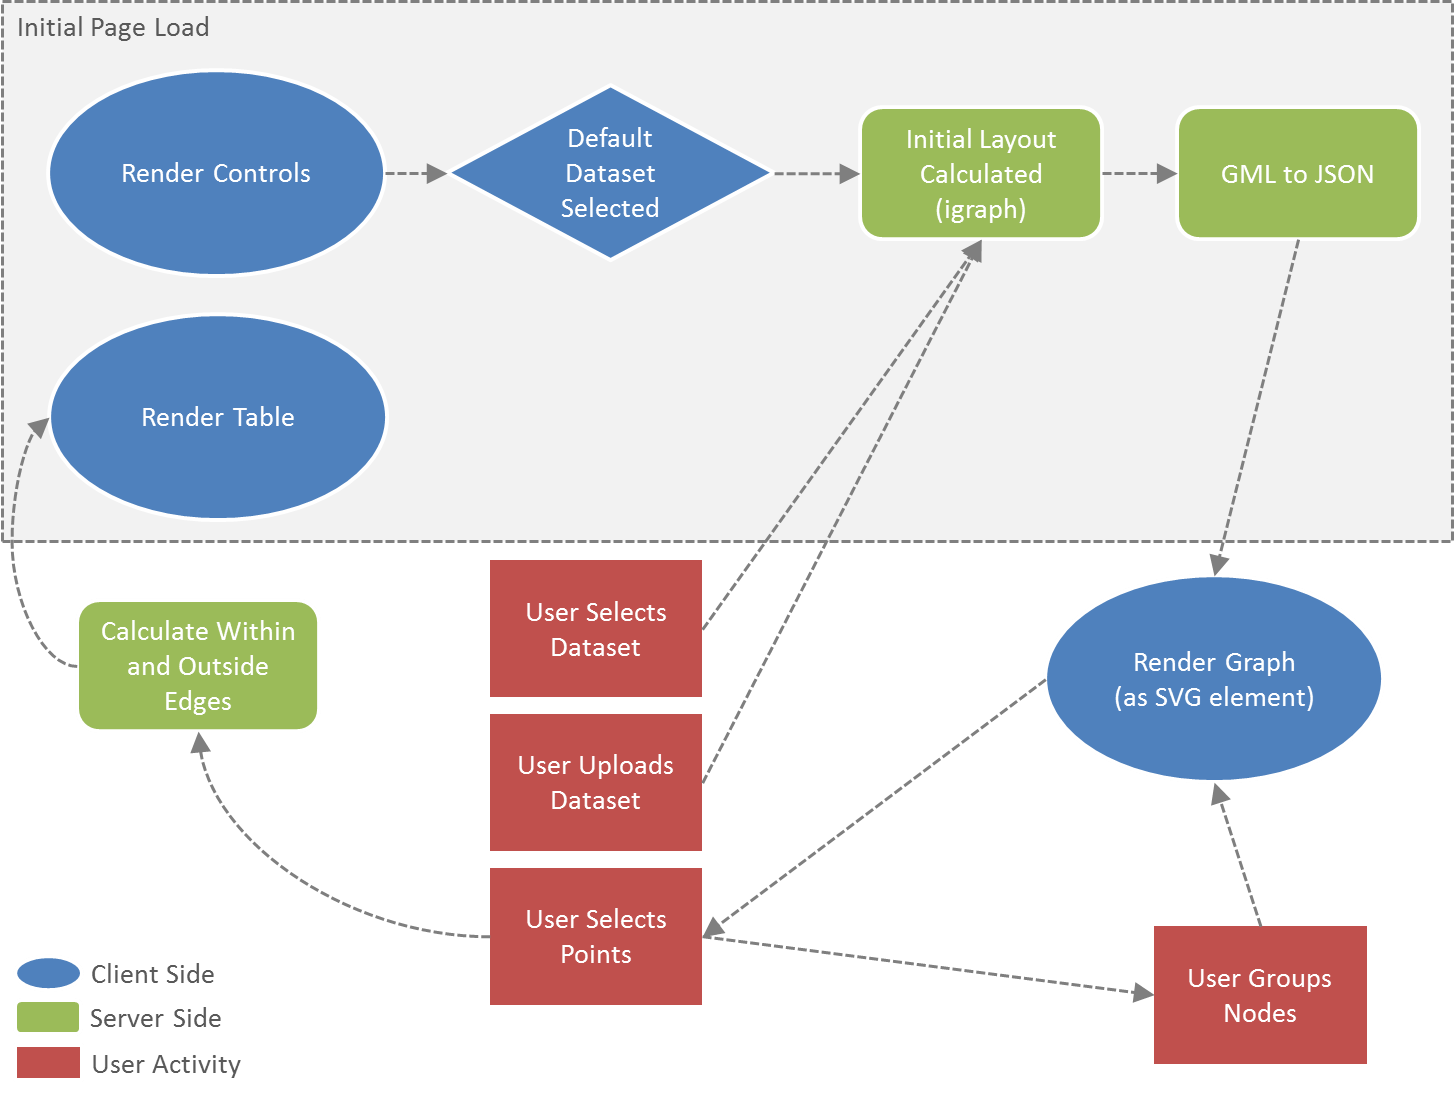
\includegraphics[width=\textwidth]{images/pagelifecycle.png}
\caption{\label{fig:pagelifecycle} Page lifecycle beginning from on load. User actions are highlighted in red, server actions in green, and actions completed on the client side are highlighted in blue. \hh{Why is there an arrow from the graph to the user?}}
\end{figure}


\paragraph{igraph}

igraph \cite{gc-igraph} is a software package used for creating and manipulating undirected and directed graphs. It is a cross-language package available for C, R, python, and Ruby. igraph also supports multiple graph file formats and visualization of graph structures.

gravicom utilizes two parts of igraph, first is the conversion from a gml file to an XML file. The gml file format, short for Graph Modelling Language, is a hierarchical ASCII-based file format for describing graphs. Below is an example gml file of an undirected graph consisting of two nodes linked by a single edge. The important points to note are that  node identifiers (id) have to be numeric. An edge consists only of source and target ids of the nodes it connects, while  nodes can have other attributes, e.g.~{\tt value} in the example. \hh{For a directed graph, the parameter {\tt directed} has to be set to 1, which will result in the edge information on target and source being evaluated accordingly.}
\begin{knitrout}
\definecolor{shadecolor}{rgb}{0.969, 0.969, 0.969}\color{fgcolor}\begin{kframe}
\begin{verbatim}
## graph
## [
##   directed 0
##   node
##   [
##     id 0
##     label "Node 1"
##     value 100
##   ]
##   node
##   [
##     id 1
##     label "Node 2"
##     value 200
##   ]
##   edge
##   [
##     source 1
##     target 0
##   ]
## ]
\end{verbatim}
\end{kframe}
\end{knitrout}

For the conversion from an  XML file  to a JSON file we make user of the R package {\tt rjson} \cite{acb-rjson}.  JSON is the native data format used in D3, which  makes working with data in the D3 library incredibly straightforward. Here is our example in the finalized JSON format:
\begin{knitrout}
\definecolor{shadecolor}{rgb}{0.969, 0.969, 0.969}\color{fgcolor}\begin{kframe}
\begin{verbatim}
## {
##   "nodes":
##   [{"id":"n0","v_id":"0","v_label":"Node 1","v_value":"100"}, 
##    {"id":"n1","v_id":"1","v_label":"Node 2","v_value":"200"}], 
##  "edges":
##   [{"source":0, "target":1}]
## }
\end{verbatim}
\end{kframe}
\end{knitrout}

Our example data will yield the graph in figure~\ref{fig:samplegraph}.

\begin{figure}[hbtp]
\centering
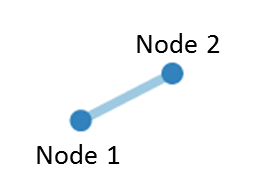
\includegraphics{images/samplegraph.png}
\caption{\label{fig:samplegraph} Graph created from sample gml file.}
\end{figure}
The second use of igraph within gravicom is to compute initial $x$ and $y$ coordinates for the nodes of the graph using a force-driven layout. This provides the initialization for the force-layout algorithm in D3. This reduces the computational load on the clients' side and helps minimize unnecessary movement by the nodes. This is critical as the extra movement at the loading of the pages creates an unnecessarily chaotic start to the user's experience. 




\subsubsection{Data Management}

\section{Further Work}

\printbibliography
\end{document}
